\documentclass[landscape,final,a0paper,fontscale=0.38]{baposter}

\usepackage{calc}
\usepackage{graphicx}
\usepackage{amsmath}
\usepackage{amssymb}
\usepackage{relsize}
\usepackage{multirow}
\usepackage{rotating}
\usepackage{bm}
\usepackage{url}
%\usepackage[brazil]{babel}   
\usepackage[utf8]{inputenc}  
\usepackage{algpseudocode}
\usepackage{algorithm}
\usepackage{graphicx}
\usepackage{multicol}
\usepackage{setspace}
\usepackage[super]{nth}
\usepackage{etoolbox} % to avoid printing "Reference" title on bibliografy command

\usepackage{lipsum}   % dummy text

% to avoid printing "Reference" title on bibliografy command
\patchcmd{\thebibliography}{\section*{\refname}}{}{}{}

%\usepackage{times}
%\usepackage{helvet}
%\usepackage{bookman}
\usepackage{palatino}

\usepackage{mdframed}    % para adicionar margem ao redor do texto nos quadros
\usepackage{xcolor}
\usepackage{color}    % para definir novas cores

%\setlength\FrameSep{0.5em}
%\setlength\OuterFrameSep{\partopsep}

\newcommand{\captionfont}{\footnotesize}
\newcommand{\mymathstyle}{\textstyle}

%  WCCI pallet
\definecolor{wcci1}{HTML}{FD6C62} % red
\definecolor{wcci2}{HTML}{FCA43B} % orange
\definecolor{wcci3}{HTML}{AED975} % green
\definecolor{wcci4}{HTML}{AAC1DA} %
%\colorlet{wcci4}{black!30} % gray


\colorlet{wcci1b}{wcci1!60}
\colorlet{wcci2b}{wcci2!60}
\colorlet{wcci3b}{wcci3!60}
\colorlet{wcci4b}{wcci4!60}

\colorlet{wcci1bg}{white}
\colorlet{wcci2bg}{white}
\colorlet{wcci3bg}{white}
\colorlet{wcci4bg}{white}

\newenvironment{cframed}[1][white]
  {\begin{mdframed}[linewidth=0,backgroundcolor=#1] }
  {\end{mdframed}}

%\graphicspath{{images/}{../images/}}
\usetikzlibrary{calc}
\newcommand{\scecore}{SCEcr}
\newcommand{\fvar}[1]{{\tiny(#1)}}
\newcommand{\myBoxEnv}[2]{\begin{cframed}[#1] #2 \end{cframed}}

\newcommand{\SET}[1]  {\ensuremath{\mathcal{#1}}}
\newcommand{\MAT}[1]  {\ensuremath{\boldsymbol{#1}}}
\newcommand{\VEC}[1]  {\ensuremath{\boldsymbol{#1}}}
\newcommand{\Video}{\SET{V}}
\newcommand{\video}{\VEC{f}}
\newcommand{\track}{x}
\newcommand{\Track}{\SET T}
\newcommand{\LMs}{\SET L}
\newcommand{\lm}{l}
\newcommand{\PosE}{\SET P}
\newcommand{\posE}{\VEC p}
\newcommand{\negE}{\VEC n}
\newcommand{\NegE}{\SET N}
\newcommand{\Occluded}{\SET O}
\newcommand{\occluded}{o}

\newcommand{\ts}{\textsuperscript}
\newcommand{\spc}{\phantom{a}}

%%%%%%%%%%%%%%%%%%%%%%%%%%%%%%%%%%%%%%%%%%%%%%%%%%%%%%%%%%%%%%%%%%%%%%%%%%%%%%%%
%%%% Some math symbols used in the text
%%%%%%%%%%%%%%%%%%%%%%%%%%%%%%%%%%%%%%%%%%%%%%%%%%%%%%%%%%%%%%%%%%%%%%%%%%%%%%%%

%%%%%%%%%%%%%%%%%%%%%%%%%%%%%%%%%%%%%%%%%%%%%%%%%%%%%%%%%%%%%%%%%%%%%%%%%%%%%%%%
% Multicol Settings
%%%%%%%%%%%%%%%%%%%%%%%%%%%%%%%%%%%%%%%%%%%%%%%%%%%%%%%%%%%%%%%%%%%%%%%%%%%%%%%%
\setlength{\columnsep}{1.5em}
\setlength{\columnseprule}{0mm}

%%%%%%%%%%%%%%%%%%%%%%%%%%%%%%%%%%%%%%%%%%%%%%%%%%%%%%%%%%%%%%%%%%%%%%%%%%%%%%%%
% Save space in lists. Use this after the opening of the list
%%%%%%%%%%%%%%%%%%%%%%%%%%%%%%%%%%%%%%%%%%%%%%%%%%%%%%%%%%%%%%%%%%%%%%%%%%%%%%%%
\newcommand{\compresslist}{%
\setlength{\itemsep}{1pt}%
\setlength{\parskip}{0pt}%
\setlength{\parsep}{0pt}%
}

%%%%%%%%%%%%%%%%%%%%%%%%%%%%%%%%%%%%%%%%%%%%%%%%%%%%%%%%%%%%%%%%%%%%%%%%%%%%%%
%%% Begin of Document
%%%%%%%%%%%%%%%%%%%%%%%%%%%%%%%%%%%%%%%%%%%%%%%%%%%%%%%%%%%%%%%%%%%%%%%%%%%%%%

\begin{document}

%%%%%%%%%%%%%%%%%%%%%%%%%%%%%%%%%%%%%%%%%%%%%%%%%%%%%%%%%%%%%%%%%%%%%%%%%%%%%%
%%% Here starts the poster
%%%---------------------------------------------------------------------------
%%% Format it to your taste with the options
%%%%%%%%%%%%%%%%%%%%%%%%%%%%%%%%%%%%%%%%%%%%%%%%%%%%%%%%%%%%%%%%%%%%%%%%%%%%%%
% Define some colors

%\definecolor{lightblue}{cmyk}{0.83,0.24,0,0.12}
\definecolor{lightblue}{rgb}{0.145,0.6666,1}

% Draw a video
\newlength{\FSZ}
\newcommand{\drawvideo}[3]{% [0 0.25 0.5 0.75 1 1.25 1.5]
   \noindent\pgfmathsetlength{\FSZ}{\linewidth/#2}
   \begin{tikzpicture}[outer sep=0pt,inner sep=0pt,x=\FSZ,y=\FSZ]
   \draw[color=lightblue!50!black] (0,0) node[outer sep=0pt,inner sep=0pt,text width=\linewidth,minimum height=0] (video) {\noindent#3};
   \path [fill=lightblue!50!black,line width=0pt] 
     (video.north west) rectangle ([yshift=\FSZ] video.north east) 
    \foreach \x in {1,2,...,#2} {
      {[rounded corners=0.6] ($(video.north west)+(-0.7,0.8)+(\x,0)$) rectangle +(0.4,-0.6)}
    }
;
   \path [fill=lightblue!50!black,line width=0pt] 
     ([yshift=-1\FSZ] video.south west) rectangle (video.south east) 
    \foreach \x in {1,2,...,#2} {
      {[rounded corners=0.6] ($(video.south west)+(-0.7,-0.2)+(\x,0)$) rectangle +(0.4,-0.6)}
    }
;
   \foreach \x in {1,...,#1} {
     \draw[color=lightblue!50!black] ([xshift=\x\linewidth/#1] video.north west) -- ([xshift=\x\linewidth/#1] video.south west);
   }
   \foreach \x in {0,#1} {
     \draw[color=lightblue!50!black] ([xshift=\x\linewidth/#1,yshift=1\FSZ] video.north west) -- ([xshift=\x\linewidth/#1,yshift=-1\FSZ] video.south west);
   }
   \end{tikzpicture}
}

\hyphenation{resolution occlusions}
%%
\begin{poster}%
  % Poster Options
  {
  % Show grid to help with alignment
  grid=false,
  % Column spacing
  colspacing=1.5em,
  % Color style
  bgColorOne=white,
  bgColorTwo=white,
  borderColor=black,
  headerColorOne={rgb:red,30;green,146;blue,154},
  headerColorTwo={rgb:red,30;green,146;blue,154},
  headerFontColor=black,
  boxColorOne=white,
  boxColorTwo={rgb:red,30;green,146;blue,154},
  % Format of textbox
  textborder=roundedleft,
  % Format of text header
  eyecatcher=true,
  headerborder=closed,
  headerheight=0.1\textheight,
%  textfont=\sc, An example of changing the text font
  headershape=roundedright,
  headershade=shadelr,
  headerfont=\Large\bf\textsc, %Sans Serif
  textfont={\setlength{\parindent}{1.5em}},
  boxshade=plain,
%  background=shade-tb,
  background=plain,
  linewidth=2pt
  }
  % Eye Catcher
  {
\includegraphics[height=8em]{imgs/wcci-logo}} 
  % Title
  {\bf\textsc{\LARGE \fontsize{19pt}{0.5cm}\selectfont A shuffled complex evolution algorithm for
the multidimensional knapsack problem using core concept}\vspace{0.3em}}
  % Authors
  %{\textsc{\{dluchi,wsantos,arodrigues,fvarejao\}@ninfa.inf.ufes.br}}
{\textsc{Marcos Baroni \& Flávio Varejão \\ \vspace{0.1em} {\large Universidade Federal do Es\'irito Santo, Vit\'oria, ES, Brazil} }}
  % University logo
  {% The makebox allows the title to flow into the logo, this is a hack because of the L shaped logo.
    
\includegraphics[height=8.0em]{../../brasao-ufes}
  }

%
% A coloured circle useful as a bullet with an adjustably strong filling
\newcommand{\colouredcircle}{%
  \tikz{\useasboundingbox (-0.2em,-0.32em) rectangle(0.2em,0.32em); \draw[draw=black,fill=lightblue,line width=0.03em] (0,0) circle(0.18em);}}

\headerbox{The Problem (MKP)}
  {headerColorOne=wcci1,headerColorTwo=wcci1b,boxColorOne=wcci1bg,name=mkp,column=0,row=0}
  {\myBoxEnv{wcci1bg}{The multidimensional knapsack problem (MKP) is a strongly NP-hard combinatorial
optimization problem which can be viewed as a resource allocation problem and
defined as follows:
\vspace{-15pt}
\begin{align*}
    \text{max} ~ & {\mymathstyle \sum_{j=1}^n p_j x_j} \\[3pt]
    \text{s. to} ~ & {\mymathstyle \sum_{j=1}^n w_{ij} x_j \leqslant c_i \quad i \in \{1, \ldots, m\}}\\
   & x_j \in \{0, 1\}, \quad j \in \{1, \ldots, n\}.
\end{align*}
\vspace{30pt}
The work address the application of a metaheuristic called
shuffled complex evolution (SCE) to the MKP.
}}

\headerbox{The Meta-heuristic (SCE)}
  {headerColorOne=wcci2,headerColorTwo=wcci2b,boxColorOne=wcci2bg,name=sce,column=0,below=mkp}
  {\myBoxEnv{wcci2bg}{The {\bf shuffled complex evolution} (SCE) \cite{duan1992effective}
is a population
based evolutionary optimization algorithm that regards a natural 
evolution happening simultaneously in $N$ independent communities (or {\bf complexes}).

Initialy $N*M$ individuals are randomly taken from the feasible solution space and
sorted according to their fitness.
Subsequently a {\bf shuffling} process places the \nth{1} in the first complex,
the \nth{2} in second complex, individual N\ts{th} goes to N\ts{th} complex,
individual $M+1$ goes back to the first complex, etc.
\vspace*{-20pt}
\begin{center}
\noindent\begin{tabular}{@{\hspace{0.0em}}c@{\hspace{1.0em}}c@{\hspace{0.0em}}}
\hspace{-3mm}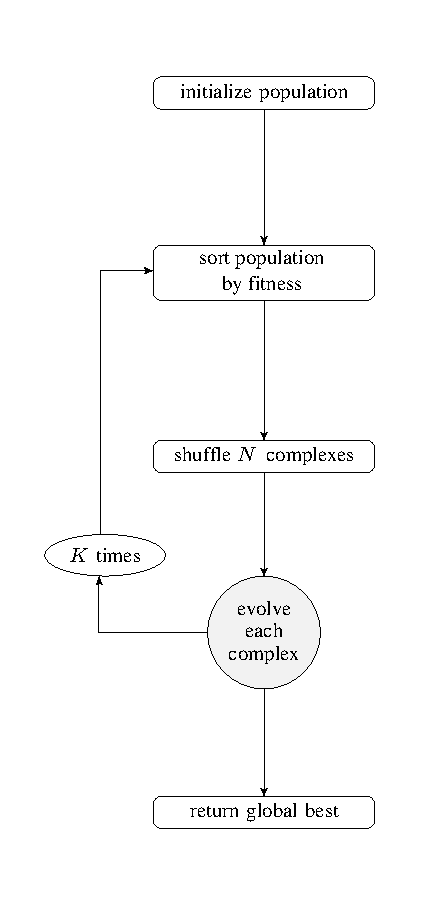
\includegraphics[width=0.46\linewidth]{imgs/flow1a} &
\hspace{-3mm}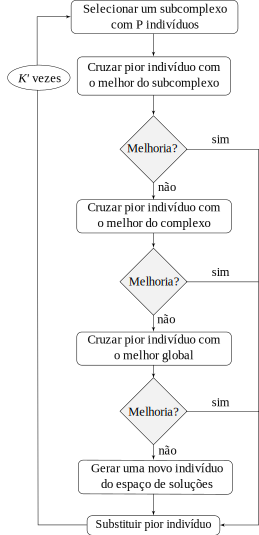
\includegraphics[width=0.46\linewidth]{imgs/flow2} \\
{\scriptsize The SCE algorithm.} & {\scriptsize Evolving stage.}
\end{tabular}
\end{center}
The next step after shuffling the complexes is to evolve each each of then through
a fixed amount of {\it (a)} $K'$ steps.
In each step {\it (b)} a {\bf subcomplex} of $P$ individuals is selected from the
complex, prioritizing those with better fitness.

The worst individual from the  subcomplex is identified to
be replaced by a new one generated by {\it (c)} its crossing 
with best individual of the subcomplex.

If the new solution has not improved {\it (d)} the best individual
of the {\bf complex} is considered for crossing and latter the {\it (e)} best one  
of whole {\bf population}.
If all the crossing steps couldn't improve the worst individual,
it is {\it (f)} replaced by a {\bf new random} solution.
 }}

\headerbox{Results}
  {headerColorOne=wcci3,headerColorTwo=wcci3b,boxColorOne=wcci3bg,name=results,column=2,span=2,row=0}
  {\myBoxEnv{wcci3bg}{Two main tests was considered.
The first one was the set of problems defined by Chu and Beasley~\cite{Chu-Beasley-1998}
and the seconf was the set composed by 11 instances defined in \cite{glover1996critical}.

Columns {\bf n} and {\bf m} indicate the size of each instance,
{\bf time} column shows the average execution time (lower is better),
{\bf quality} column shows the average ratio of the solution found and
the best known solution from literature, variance values shown in parentheses.
\\[3pt]
\begin{minipage}[c]{0.4\linewidth}
  \begin{center}
      {\bf Table I}: Performance on Chu-Beasley problems. \\[3pt]
    \begin{tabular}{|r|r|rr|rr|} \cline{3-6}
  \multicolumn{2}{c|}{} &
    \multicolumn{2}{c|}{\bf time (s)} &
    \multicolumn{2}{c|}{\bf quality (\%)} \\ \hline
  \textbf{n}   &
    \textbf{m}  &
    \textbf{SCE} &
    \textbf{\scecore} &
    {\bf SCE} &
    {\bf \scecore}  \\ \hline
100
  &  5 & 1.31\fvar{0.03} & 0.17\fvar{0.00} & 97.60\fvar{0.56} & 99.83\fvar{0.02} \\ \hline
  & 10 & 1.43\fvar{0.04} & 0.26\fvar{0.00} & 96.96\fvar{0.99} & 99.75\fvar{0.04} \\ \hline
  & 30 & 1.75\fvar{0.08} & 1.01\fvar{0.04} & 96.66\fvar{0.66} & 98.89\fvar{0.11} \\ \hline
250
  &  5& 2.87\fvar{0.09} & 0.69\fvar{0.01} & 94.98\fvar{0.33} & 99.92\fvar{0.00} \\ \hline
  & 10 & 3.08\fvar{0.09} & 0.83\fvar{0.01} & 94.95\fvar{0.35} & 99.75\fvar{0.00} \\ \hline
  & 30 & 3.82\fvar{0.14} & 1.45\fvar{0.05} & 94.65\fvar{0.39} & 98.89\fvar{0.04} \\ \hline
500 
  &  5 & 5.74\fvar{0.14} & 1.23\fvar{0.01} & 93.73\fvar{0.28} & 99.86\fvar{0.00} \\ \hline
  & 10 & 5.85\fvar{0.34} & 1.33\fvar{0.03} & 93.65\fvar{0.25} & 99.71\fvar{0.00} \\ \hline
  & 30 & 6.17\fvar{1.12} & 1.84\fvar{0.19} & 93.30\fvar{0.34} & 99.28\fvar{0.01} \\ \hline
\end{tabular}

  \end{center}
  \vfill
\end{minipage}
\begin{minipage}[c]{0.6\linewidth}
  \begin{center}
      {\bf Table II}: Performance on Glover-Kochenberger problems.  \\[3pt]
    \begin{tabular}{|r|r|r|c|r|r|r|} \cline{4-7}
  \multicolumn{3}{c|}{} &
    \multicolumn{2}{c|}{\bf time (s)} &
    \multicolumn{2}{c|}{\bf quality (\%)} \\ \hline
  \textbf{\#} &
    \textbf{n}   &
    \textbf{m}  &
    {\bf SCE } &
    {\bf SCEcr } &
    {\bf SCE} &
    {\bf SCEcr} \\ \hline
  01   &  100 &  15 &   1.47\fvar{0.00} & 0.08\fvar{0.0} & 97.66\fvar{0.03} & 99.24\fvar{0.02} \\ \hline
    02 &  100 &  25 &   1.61\fvar{0.00} & 0.09\fvar{0.0} & 97.94\fvar{0.04} & 98.94\fvar{0.09} \\ \hline
    03 &  150 &  25 &   2.51\fvar{0.01} & 0.09\fvar{0.0} & 97.22\fvar{0.04} & 99.09\fvar{0.02} \\ \hline
    04 &  150 &  50 &   3.56\fvar{0.03} & 0.09\fvar{0.0} & 97.40\fvar{0.04} & 98.52\fvar{0.02} \\ \hline
    05 &  200 &  25 &   3.55\fvar{0.01} & 0.09\fvar{0.0} & 96.88\fvar{0.03} & 99.28\fvar{0.01} \\ \hline
    06 &  200 &  50 &   4.81\fvar{0.09} & 0.10\fvar{0.0} & 97.68\fvar{0.02} & 98.90\fvar{0.03} \\ \hline
    07 &  500 &  25 &   7.30\fvar{0.09} & 0.10\fvar{0.0} & 97.12\fvar{0.01} & 99.54\fvar{0.00} \\ \hline
    08 &  500 &  50 &  12.20\fvar{0.47} & 0.11\fvar{0.0} & 97.27\fvar{0.01} & 99.33\fvar{0.01} \\ \hline
    09 & 1500 &  25 &  24.61\fvar{1.73} & 0.12\fvar{0.0} & 95.40\fvar{0.01} & 98.22\fvar{0.00} \\ \hline
    10 & 1500 &  50 &  33.79\fvar{2.44} & 0.13\fvar{0.0} & 97.50\fvar{0.00} & 99.64\fvar{0.00} \\ \hline
    11 & 2500 & 100 & 121.28\fvar{194.74} & 0.15\fvar{0.0} & 97.95\fvar{0.00} & 99.70\fvar{0.00} \\ \hline
\end{tabular}

  \end{center}
\end{minipage}
\\

It can be noticed that \scecore achieved high quality solutions, at least $98.22\%$
of best known solution, spending short amount of processing time.
 }}

\headerbox{The Core Concept for MKP}
  {headerColorOne=wcci2,headerColorTwo=wcci2b,boxColorOne=wcci2bg,name=scemkp,column=1,span=1,row=0}
  {\myBoxEnv{wcci2bg}{The core concept was first presented for the one-dimensional 0-1 knapsack problem (KP),
leading to very successful KP algorithms.
The main idea is to reduce the original problem by only considering a set of
items for which it is hard to decide if they will occur or not in an optimal solution.
This set of items is named core.
The variables for all items outside the core are fixed to certain values.

The knapsack problem considers items $j = 1, \ldots, n$, associated profits $p_j$ and
associated weights $w_j$.
A subset of these items has to be selected and packed into a knapsack having capacity $c$.
The total profit of the items in the knapsack has to be maximized, while the
total weight is not allowed to exceed $c$.

Before defining the core of the KP it is worth to note the solution structure
of its LP-relaxation.
The LP-relaxation of an integer programming problem arises by replacing the
constraint that each variable must be integer by a constraint that allows
continuity of the variable.
The LP-relaxation of a KP is found by replacing the constraint $x_i \in \{0,1\}$
by $0 \leqslant x_i \leqslant 1$ for all $i \in \{1, \ldots, n\}$.
If the items are sorted according to decreasing efficiency values
\begin{displaymath}
  e_j = \frac{p_j}{w_j},
\end{displaymath}
it is known that the solution of the LP-relaxation consists of
three consecutive parts: the first part contains variables set to $1$, the second
pare consists of at most one split item $s$, whose corresponding LP-values is
fractional, and finally the remaining variables, which are always set to zero,
form the third part.

For most instance of KP (except those with a very special structure) the integer
optimal solution closely corresponds to this partitioning in the sense that it
contains most of the highly efficient items of the first part, some items with
medium efficiencies near the split item, and almost no items with low efficiencies
from the third part.
Items of medium efficiency constitute the core.

Balas and Zemel~\cite{balas1980algorithm} gave the following precise definition
of the core of a KP, based on the knowledge of an optimal integer solution $x^*$.
Assume that the items are sorted according to decreasing efficiencies and let
\begin{displaymath}
  a := \min\{ j | x_j^* = 0 |\}, \quad b := \max\{ j | x_j^* = 1 \}.
\end{displaymath}
The core is given by the items in the interval $C = \{a, \ldots, b\}$.
It is obvious that the split item is always part of the core, i.e., $a < s < b$.

Figure~\ref{fig:kpecore} illustrates an exact core for an hypothetical KP instance
with $13$ items.
First row represents the efficiency value $e$ of each item.
The items are sorted by descending order of efficiency.
Second row represent solution array of the LP-relaxation.
The third row represents the exact solution for the original problem.
The $8$-th item is the split item.
Notice that the split item is within the exact core.

\begin{figure}[h]
  \centering
  \includegraphics[scale=0.406]{imgs/core}
  \caption{Example of exact core for a hypothetical KP instance.}
  \label{fig:kpecore}
\end{figure}

The KP Core problem (KPC) is defined as
\begin{align*}
  \text{maximize} & \sum_{j \in C} p_j x_j  + \tilde{p}\\
  \text{subject to} & \sum_{j \in C} w_{j} x_j \leqslant c - \tilde{w}\\
  & x_j \in \{0, 1\}, \quad j \in C.
\end{align*}
with $\tilde{p} = \sum^{a-1}_{j=1} p_j$ and $\tilde{w} = \sum^{a-1}_{j=1} w_j$
respectively quantifying the total profit and the total weights of items fixed as selected.
The solution of KPC would suffice to compute the optimal solution of KP, which
however, has to be already partially known to determine $C$.
Nevertheless an approximate core $C = \{s-\delta, \ldots, s+\delta\}$,
of fixed size $|C| = 2\delta+1$ is considered for a heuristic reduction of the problem.

Figure~\ref{fig:kpcore} exemplifies an approximate core of a hypothetical KP
instance with $13$ items.
The first row represents the efficiency value of each item and the second row
represents the value of each variable on the LP-relaxation optimal solution.
The items are sorted in descending order of efficiency value.
The last row illustrates the variable fixing after the defined core.
Asterisks indicate free variables associated to the items in the
approximate core.

\begin{figure}[h]
  \centering
  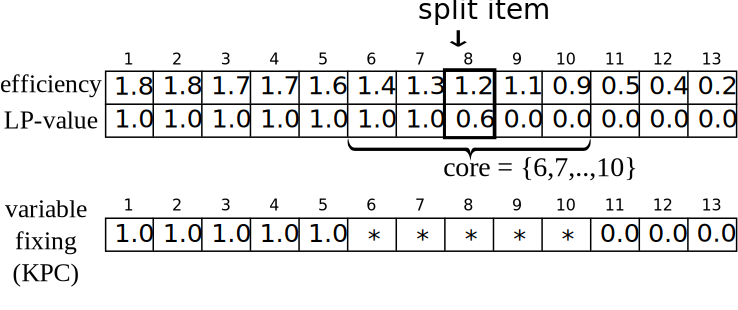
\includegraphics[scale=0.406]{imgs/kp_3}
  \caption{Example of core for a hypothetical KP instance with $n=13$ and approximate core size of $5$ ($\delta = 2$).}
  \label{fig:kpcore}
\end{figure}

\subsection{The Core Concept for MKP}

The previous definition of the core for KP can be extended to MKP without major
difficulties, once an efficiency measure is defined for the MKP,
as addressed in \cite{puchinger2006core}, even though,
a proper efficiency measure for MKP is not obvious due the
multidimensional weight of the items.
A well accepted efficiency measure is discussed in Section~\ref{subsec:dual}.

Now let $x^*$ be an optimal solution for a MKP and assume that the items are
sorted in descending order after some given efficiency measure. Then let
\begin{displaymath}
  a = \min \{ j | x_j^* = 0 \}, \quad b = \max \{ j | x_j^* = 1 \}.
\end{displaymath}
The core is given by the items in the interval $C = \{ a, \ldots, b \}$,
and the multidimensional knapsack core problem (MKPC) defined as
\begin{align*}
  \text{maximize} & \sum_{j \in C} p_j x_j  + \tilde{p}\\
  \text{subject to} & \sum_{j \in C} w_{ij} x_j \leqslant c_i - \tilde{w}_i, \quad i = 1, \ldots, m\\
  & x_j \in \{0, 1\}, \quad j \in C.
\end{align*}
with $\tilde{p} = \sum^{a-1}_{j=1} p_j$  and $\tilde{w}_i = \sum^{a-1}_{j=1} w_{ij}, i = 1, \ldots, m$.

In contrast to KP, the solution of the LP-relaxation of MKP in general does not
consists of a single fractional split item. But up to $m$ fractional values give
rise to a whole \emph{split interval} $S = \{ s_1, \ldots, s_m\}$, where
$s_1$ and $s_m$ are respectively the first and the last index of variables with
fractional values after sorting by the given efficiency measure.
Once the split interval is defined, a central index value $s = \lfloor \frac{s_1+s_m}{2}\rfloor$
can be used as the center of an approximate core.

\subsection{The Dual-variable Efficiency Measure}
\label{subsec:dual}
For defining a reasonable efficiency measure for MKP consider the most obvious
form of efficiency which is a direct generalization of the one-dimensional case:
\begin{displaymath}
	e_j(simple) = \frac{p_j}{\sum_{i=1}^{m} w_{ij}}
\end{displaymath}
In this definition different orders of magnitude of the constraints are not
considered and a single constraint may dominate the others.
This drawback can be avoided by introducing relevance values $r_i$ for every
constraint:
\begin{displaymath}
	e_j(relevance) = \frac{p_j}{\sum_{i=1}^{m} r_i w_{ij}}
\end{displaymath}
Several proposals for setting the relevance values $r_i$ were discussed and
tested by Puchinger, Raidl and Pferschy in \cite{puchinger2006core}.
According to their work setting the relevance values $r_i$ to the values of an
optimal solution to the dual problem of the MKP's LP-relaxation, as suggested
in \cite{Chu-Beasley-1998}, achieved the best results and will be the one
considered in this work for the development of the hybrid heuristic.

While the original MKP can be seen as a resource allocation problem,
the dual problem of the MKP can be seen as a resource valuation problem.
For this reason the values of the dual solution is related to the
\emph{importance} of each resource.

The split interval resulting from the efficient measure considered can be
precisely characterized.
Let $x^{LP}$ be the optimal solution of the LP-relaxation of MKP.
Then the following relation holds, as proved in \cite{puchinger2006core}:
\begin{displaymath}
 x_l^{LP} =
  \begin{cases}
    1         & \mbox{if } e_j > 1, \\
    \in [0,1] & \mbox{if } e_j = 1, \\
    0         & \mbox{if } e_j < 1.
  \end{cases}
\end{displaymath}
From this relation we can note that all variables in the split interval will
have efficiency measure $e_j = 1$, while less and more efficient ones will have
$e_j < 1$ and $e_j > 1$ respectively.

Figure~\ref{fig:mkpcore} exemplifies an approximate core of a hypothetical MKP
with $13$ variables and $3$ dimensions.
Notice that the LP-relaxation solution has now $3$ fractional variables that
defines the center of the split interval.

\begin{figure}[h]
  \centering
  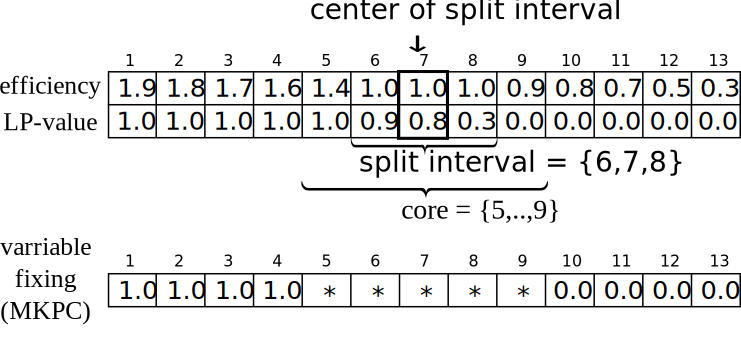
\includegraphics[scale=0.406]{imgs/mkp_3}
  \caption{Example of core for a hypothetical MKP instance with $n=13$, $m=3$ and approximate core size of $5$ ($\delta = 2$).}
  \label{fig:mkpcore}
\end{figure}

The following section presents the shuffled complex evolution algorithm
and proposes its application on the MKP.
}}

\headerbox{The SCE for MKP}
  {headerColorOne=wcci2,headerColorTwo=wcci2b,boxColorOne=wcci2bg,name=scemkp,column=1,span=2,row=0,above=bottom}
  {\myBoxEnv{wcci2bg}{As it can be noted in its description the SCE is easly applied to any
optimization problem.
The only steps needed to be specified is the creation of a {\bf new MKP random
solution} (Algorithm 1) and the {\bf crossing procedure of two MKP solutions} (Algorithm 2).
\begin{center}
\hspace*{-28pt}
\begin{minipage}[c]{0.5\linewidth}
  \begin{center}
    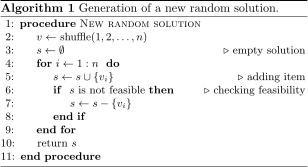
\includegraphics[width=0.87\linewidth]{imgs/alg-new}\\[3mm]
  \end{center}
\end{minipage}
\begin{minipage}[c]{0.4\linewidth}
  \begin{center}
    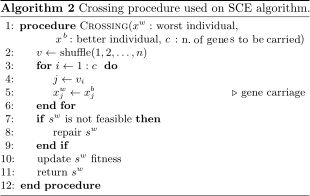
\includegraphics[width=0.95\linewidth]{imgs/alg-cross}
  \end{center}
\end{minipage}
\end{center}
%\vspace{0.1mm}
 }}

\headerbox{Experimental Setup}
  {headerColorOne=wcci3,headerColorTwo=wcci3b,boxColorOne=wcci3bg,name=setup,column=2,row=0,below=results} {\myBoxEnv{wcci3bg}{Several computational experiments was executed to verify the efficiency of the
hybrid method (\scecore) over the original SCE proposed in
\cite{baroni2015shuffled} (SCE).
In all instances the {\bf parameters} used for SCE and \scecore were the same recommended
in \cite{baroni2015shuffled} which was found after a batch test using Chu and Beasley instances:

\begin{center}
  \resizebox{0.9\columnwidth}{!}{%
  \begin{tabular}{|c|c|l|}
  \hline
  \multicolumn{1}{|c}{\rule{0pt}{12pt} \spc } & \multicolumn{1}{|c|}{\bf \spc Value \spc } & \multicolumn{1}{c|}{\bf Description} \\[2pt]
  \hline\rule{0pt}{12pt}
  $N$  & $20$  & \spc \# of complexes \\
  $M$  & $20$  & \spc \# of individuals in each complex \\
  $P$  & $5$   & \spc \# of individuals in each subcomplex \\
  $K$  & $300$ & \spc \# of algorithm iterations \\
  $K'$ & $20$  & \spc \# of iterations of evolving process \\
  $c$  & $n/5$ & \spc \# of genes carried from parent in crossing \\[2pt]
  \hline
  \end{tabular}
}


\end{center}

The experiments were run on a 3.40GHz computer with 4GB of RAM.
The algorithms was implemented in C programming language.
 }}

\headerbox{Conclusions \& Future Remarks}
  {headerColorOne=wcci4,headerColorTwo=wcci4b,boxColorOne=wcci4bg,name=conclusions,column=3,below=results}
  {\myBoxEnv{wcci4bg}{In this work we addressed the application of the shuffled complex
evolution (SCE) to the multidimensional knapsack problem and investigated it
performance through several computational experiments.

The SCE algorithm, which combines the ideas of a controlled random search with
the concepts of competitive evolution proved to be very effective in finding
good solution for hard instances of MKP, demanding a very small amount of
processing time to reach high quality solutions for MKP.
 Future work includes the investigation of different crossing procedures,
the use of local search in the process of evolving complexes and the
application of problem reduction procedures for the MKP.

 }}

%\headerbox{Future Remarks}
%  {headerColorOne=wcci4,headerColorTwo=wcci4b,boxColorOne=wcci4bg,name=future,column=3,below=conclusions}
%  {\myBoxEnv{wcci4bg}{Future work includes the investigation of different crossing procedures,
the use of local search in the process of evolving complexes and the
application of problem reduction procedures for the MKP.

 }}

\headerbox{References}
  {headerColorOne=wcci4,headerColorTwo=wcci4b,boxColorOne=wcci4bg,name=references,column=3,below=conclusions}
  {\small \bibliographystyle{plain} \bibliography{../../../refs} }

\headerbox{Acknowledgement}
  {headerColorOne=wcci4,headerColorTwo=wcci4b,name=acknowledgement,column=3,above=bottom}
  {\fontsize{8pt}{0.5cm}\selectfont Research supported by Funda\c c\~ao de Amparo \`a Pesquisa do Esp\'irito Santo.  }

\end{poster}

\end{document}

